\documentclass[12pt]{article}
\usepackage{mathtools}
\usepackage[papersize={210mm, 270mm},tmargin=17mm,bmargin=15mm,lmargin=15mm,rmargin=15mm]{geometry}
\usepackage[utf8]{inputenc}
\usepackage{graphicx}
\usepackage{fancyhdr}
\usepackage{tikz}
\usepackage{listings}
\usetikzlibrary{positioning}
\usetikzlibrary{arrows.meta, automata, positioning, quotes}
\pagestyle{fancy}
\lhead[\thepage]{David Cuesta Martín}
\rhead[David Cuesta Martín]{\thepage}
\cfoot{}
\author{David }


\begin{document}
\section*{Ejercicio 1: }\\ \\ 
\textbf{a) }Sea $M=(\{q_0, q_1, q_2\},\{a,b\},\delta, q_0,\{q_2\})$\\ 
\begin{table}[h!]
    \begin{tabular}{c|c|c}
      $\delta(q,\sigma)$ & $a$ & $b$\\
      \hline
      $q_0$& $q_2$ & $q_1$\\
      \hline
      $q_1$& $q_1$ & $q_1$\\
      \hline
      $q_2$& $q_1$ & $q_1$
    \end{tabular}
\end{table}\\
Por tanto el dirigrafo que representa al autómata es:
\begin{center}
  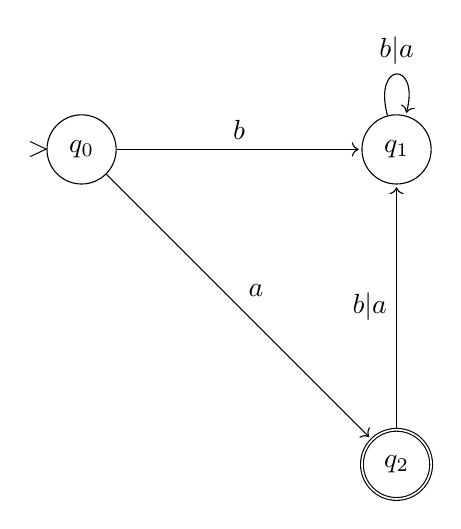
\begin{tikzpicture}[auto,
      shorten > = 1pt, 
  node distance = 4cm and 3cm]
  \node[state] (q0) {$q_0$};
  \node[inner sep=0pt,outer sep=-1pt,left=0pt of q0.west]{$>$};
  \node[state] (q1) [right of=q0] {$q_1$};
  \node[state,accepting] (q2) [below of=q1] {$q_2$};
  \path[->] (q0) edge ["$b$"] (q1)
                 edge ["$a$"] (q2)
            (q1) edge [loop above, "$b|a$"] ()
                 
            (q2) edge ["$b|a$"] (q1);
  \end{tikzpicture}
\end{center}
\textbf{b) }Con el programa JFLAP comprobamos el grafo descrito con 6 cadenas:
\begin{center}
    \includegraphics[width=17cm]{img1.png}
\end{center}
\newpage
\section*{Ejercicio 2: }
\textbf{a) }Probamos la función definida en el repositorio:
\begin{center}
    \includegraphics[width=16cm]{img2.png}
\end{center}
Una vez ya sabemos como funciona, definimos el autómata desde el archivo llamado "finiteautomata.json" tal como:
\begin{verbatim}
    [
  {
    "name" : "a*bb*aa*",
    "representation" : {
      "K" : ["q0", "q1", "q2", "q3"],
      "A" : ["a", "b"],
      "s" : "q0",
      "F" : ["q2"],
      "t" : [["q0", "a", "q0"],
             ["q0", "b", "q1"],
             ["q1", "a", "q2"],
             ["q1", "b", "q1"],
             ["q2", "a", "q2"],
             ["q2", "b", "q3"],
             ["q3", "a", "q3"],
             ["q3", "b", "q3"]]
      }
  },
  {
    "name" : "aa*bb*",
    "representation" : {
      "K" : ["q0", "q1", "q2"],
      "A" : ["a", "b"],
      "s" : "q0",
      "F" : ["q2"],
      "t" : [["q0", "a", "q1"],
             ["q1", "a", "q1"],
             ["q1", "b", "q2"],
             ["q2", "b", "q2"]]
      }
  },
  {
    "name" : "even_number_of_ones",
    "representation" : {
      "K" : ["q0", "q1"],
      "A" : ["0", "1"],
      "s" : "q0",
      "F" : ["q0"],
      "t" : [["q0", "0", "q0"],
             ["q0", "1", "q1"],
             ["q1", "0", "q1"],
             ["q1", "1", "q0"]]
      }
  },
  {
    "name" : "odd_number_of_zeroes",
    "representation" : {
      "K" : ["q0", "q1"],
      "A" : ["0", "1"],
      "s" : "q1",
      "F" : ["q0"],
      "t" : [["q0", "0", "q1"],
             ["q0", "1", "q0"],
             ["q1", "0", "q0"],
             ["q1", "1", "q1"]]
      }
  },
  {
    "name" : "lenguaje_con_a",
    "representation" : {
      "K" : ["q0", "q1", "q2"],
      "A" : ["a", "b"],
      "s" : "q0",
      "F" : ["q2"],
      "t" : [["q0", "a", "q2"],
             ["q0", "b", "q1"],
             ["q1", "a", "q1"],
             ["q1", "b", "q1"],
             ["q2", "a", "q1"],
             ["q2", "b", "q1"]]
      }
  }
]
\end{verbatim}
Una vez ya definido, ya lo podemos utilizar en nuestro programa Octave con la función ya definida "finiteautomata()":
\begin{center}
    \includegraphics[width=15cm]{img3.png}
\end{center}
Como vemos, lo he probado con 5 cadenas y la función nos dice que el autómata solo acepta, entre las cadenas introducidas, la cadena compuesta por una única a.
\end{document}
